% !TeX spellcheck = en_US
%Publications.tex
\newcommand{\PublicationsPath}{PatentsAndPublications/Publications}

%BMSB2019

\section[QoE-based enhancements of Chunked CMAF over low latency video streams]{QoE-based enhancements of Chunked CMAF over low latency video streams}
\label{chap:BMSB2019}
\begin{itemize} \itemsep1pt\parskip0pt\parsep0pt
	\item \textbf{Title:} QoE-based enhancements of Chunked CMAF over low latency video streams
	\item \textbf{Authors:} Roberto Viola, Alvaro Gabilondo, \'Angel Mart\'in, Juan Felipe Mogoll\'on and Mikel Zorrilla
	\item \textbf{Proceedings:} 2019 IEEE International Symposium on Broadband Multimedia Systems and Broadcasting (BMSB)
 	\item \textbf{Publisher:} IEEE
	\item \textbf{Year:} 2019
	\item \textbf{DOI:}  \url{10.1109/BMSB47279.2019.8971894}
\end{itemize}	

\textbf{Abstract:} 5G infrastructures are in the roadmap of content delivery services, aiming to forward all broadcast and broadband video traffic using a common telecommunication network architecture. Streaming services will benefit from 5G networks which promise higher capacity, higher bandwidth and lower latency than current infrastructures. However, the widely employed streaming technologies, such as Dynamic Adaptive Streaming over HTTP (MPEG-DASH), require an intrinsic high latency of tens of seconds to enforce the Quality of Experience (QoE). These conditions turn MPEG-DASH unfavourable when compared with a traditional broadcast pipeline for live events in terms of latency. Therefore, improvements on latency of streaming technologies are necessary to deliver live broadcast services over 5G networks. The media industry proposed a Chunked Common Media Application Format (Chunked CMAF) in order to achieve latency under a second. In this paper, we show an implementation of a Chunked CMAF for MPEG-DASH live videos in a real deployment. To further evaluate the benefits of CMAF we evaluate the QoE results when delivering a legacy MPEG-DASH live content compared to a Chunked CMAF-powered one.

\textbf{Keywords:} Chunked CMAF, Future broadcasting services, MPEG-DASH, Quality of Experience, Video coding and processing.

\subsection{Introduction}
% no \IEEEPARstart
Video streaming services represent a large fraction of the Internet traffic. In fact, live video traffic will grow 3-fold from 2017 to 2022, accounting the 17\% of all internet video traffic \cite{ciscovideo2017}. This trend would be fuelled by the deployment of 5G networks, which will enable the cooperation between broadband and broadcast services \cite{calabuig2015}.

5G networks promise high capacity, high bandwidth and low latency to cope with demanding traffic and services. Nevertheless, MPEG-DASH and other HTTP-based alternatives require to packetize video contents in segments with a duration in the order of seconds to enforce the QoE, leading to tens of seconds of delay between content generation and consumption \cite{lohmar2011}. This delay is produced by the duration of packaged media segments, designed to match changeable network delivery performance, and the required buffering, done by the media player to achieve a smooth playback for \mbox{on-demand} and live streams. This delay is not significant for \mbox{on-demand} contents, but it is too high to deliver live streams with comparable performance to the broadcast live services. Moreover, when deploying hybrid broadcast broadband services, the common mechanism to synchronize broadcast and broadband signals consists in delaying the broadcast source as broadband stream is usually 30-40 seconds delayed with respect to the broadcast service.

The Common Media Application Format (CMAF) \cite{hughes2017information}, proposed by ISO/IEC, is the solution for delivering live contents from media industry. CMAF includes two major benefits. First, it ensures the use of the ISO Base Media File Format, usually referred as MP4, as a common file format when combined with different streaming technologies such as MPEG-DASH or HTTP Live Streaming (HLS). This feature makes media storage more efficient as different manifests (MPD for MPEG-DASH and M3U8 for HLS) may index the same segments. Each media client can download a different manifest depending on its supported streaming technologies. Then, it plays the content by downloading the same media segments. Thus, the server needs lower storage capacity. Secondly, it defines a chunked mode, named Chunked CMAF or Low Latency CMAF, which enables latency enhancement of the stream, reducing the time elapsed between media packaging and its playback.

\begin{figure}[htp]
	\centering
	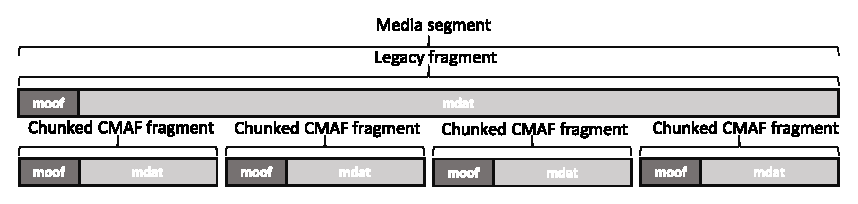
\includegraphics[width=1\textwidth,keepaspectratio]{CMAF.eps}
	\caption{Legacy fragment and Chunked CMAF fragment.}
	\label{fig:BMSB2019fragment}
\end{figure}

Typical MPEG-DASH media segments contain a single MP4 fragment with the fragment duration equal to the segment duration. Here, common values for segment duration are from 2 to 30 seconds. On the contrary, Chunked CMAF enables a single segment to contain multiple fragments as depicted in Figure \ref{fig:BMSB2019fragment}. Therefore, Chunked CMAF exploits the use of short MP4 fragments, including the minimum data required by the player to start decoding the stream. Therefore, the shorter fragment duration allows a promptly playback start, removing the limitation to fully download the entire segment. 

This work proposes a real implementation of a server-client solution delivering Chunked CMAF streams of live contents. This solution has been achieved by providing two relevant contributions:
\begin{itemize}
	\item Chunked CMAF has been integrated with an Open Source MPEG-DASH framework.
	\item The evaluation measures the effects on user's QoE while varying the fragment duration of the Chucked CMAF segments and the resulting latency.
\end{itemize}

The remainder of this paper is organized as follows. First, section \ref{sec:BMSB2019related} presents the background of the MPEG-DASH standard and Chunked CMAF for deploying live media services. Then, section \ref{sec:BMSB2019implementation} shows the implementation of Chunked CMAF solution. In section \ref{sec:BMSB2019results} we describe the experiments and present the results. Finally, in section \ref{sec:BMSB2019conlusion} we expose the conclusions and future work.

\subsection{Related Work}
\label{sec:BMSB2019related}
In this section, it is included an overview of MPEG-DASH for live streaming services and afterwards, a comprehensive review about the State of Art of Chunked CMAF is described.

\subsubsection{Overview of Live MPEG-DASH}
\label{sec:BMSB2019dash}
MPEG-DASH was developed by MPEG and standardized by ISO/IEC. In MPEG-DASH, first, the client fetches a Media Presentation Description (MPD) and parses it to be aware of the different representations of the content. Then, the player chooses the representation that fits in the device capabilities in terms of resolution, language, codec and bitrate. Accordingly, the client requests and downloads the corresponding segment from the server. Once a segment has been played, the next one from the MPD is requested. During the playback, the player can switch to a different representation depending on its preferences and network performance in order to minimize any impact on the QoE.

The live playback is possible through the \textit{availabilityStartTime} field in the MPD, which marks the UTC time when the stream is made available. The client continuously compares it with the current time to fetch the last available segments. In the case of a legacy live MPEG-DASH content, the \textit{availabilityStartTime} has to correspond to the time when the first media segment is fully available on server side. Then, the segment duration, which ranges from 2 to 30 seconds, is the minimum delay that a client experiences during a live stream. Encoding and network latency also influence this delay, but their weights in the resulting latency are 10-100ms when aggregated to the segment duration.

\subsubsection{Chunked CMAF}
\label{sec:BMSB2019cmaf}
The latency is a key factor when dealing with live streaming contents. Current MPEG-DASH-based solutions are not able to operate with a similar latency to the current broadcast solutions. This is a major challenge when targeting broadcast levels of QoE. The use of Chunked CMAF, together with improved network bandwidth and latency of the 5G networks, aims to reduce live streaming latency and keep it behind a second \cite{bouzakaria2014overhead}.

Contrary to the legacy MPEG-DASH streams, a Chunked CMAF-compliant MPEG-DASH distinguishes between MP4 fragment duration and media segment duration with different values. The reduction of the fragment duration makes the media units of the stream quickly available enabling prompt playback. Consequently, the segment contains multiple fragments and the \textit{availabilityStartTime} attribute contained in the MPD must be set at the time the first fragment is available, even if the segment is not completely written. The smaller the fragment is, the smaller delay is experienced by the player. Theoretically, fragment duration can be reduced to one frame duration. To this end, it is required a proper server, which must be able to split the HTTP response sending fragment units instead of the full segment.

Several implementations serve Chunked CMAF with \mbox{HTTP 1.1} Chunked Transfer Encoding. The server encapsulates each MP4 fragment in a HTTP chunk and deliver it over time, instead of sending the entire segment at once. In \cite{saminathan2011}, Chunked Transfer Encoding allows a \mbox{HTTP 1.1} server to split the response in small HTTP chunks. The paper shows that the latency does not depend on the segment duration but depends on the duration chosen for the HTTP chunks. This approach still uses one second duration chunks while splitting the HTTP connection between server and player. The author of \cite{essaili2018} also implements a MPEG-DASH delivery involving Chunked CMAF, but it varies the duration of the fragment. Both papers provide performance results in terms of overall latency.

The work shown in \cite{wei2014} uses HTTP 2.0 to exploit the \mbox{push-mode} added in the new HTTP version for reducing the latency. HTTP 2.0 does not have a Chunked Transfer \mbox{Encoding} mode, since it already employs a frame-based \mbox{delivery}, i.e. it splits the response in several frames which contain the Chunked CMAF MP4 fragments. This solution has the \mbox{advantage} of reducing the protocol header overhead since HTTP 2.0 header is simplified when compared to HTTP 1.1. However, push-mode reduces the adaptation possibilities at the client-side to dynamically select an appropriate representation for the network performance conditions. Decisions can be still done by the server, modifying the MPD, but this approach does not scale as the player-side decisions when working in pull-mode.

\subsubsection{QoE Metrics}

The reduction of the latency of the service is the major goal to all these scientific approaches. Nevertheless, when evaluating streaming services, it is essential to focus in user's QoE. The QoE is a key aspect for user satisfaction and retention when rating streaming services. Hence, any solution trying to enhance media delivery needs to consider QoE metrics. No one of the above works consider QoE as a metric in order to evaluate the real benefits to end users.

A commonly used scale to evaluate QoE is the Mean Opinion Score (MOS) which consists of five increasing quality levels (from 1 to 5) \cite{Itu2016}. In the literature many models are available to profile the subjective human perception of the quality and estimate the MOS through objective metrics. In \cite{claeys2014} the author uses metrics like initial delay, stalling time, number of representation switches and inter-switching times in order to get an estimated Mean Opinion Score (eMOS). This eMOS quantifies the quality of video streaming services based on objective streaming connectivity and buffering measures of players without a demographic perception study of users. In \cite{hossfeld2012} the author proposes to evaluate the MOS depending on the initial delay and the numbers of freezes. It concludes that is preferable a higher initial delay than freezes in order to have a better human perception. Recently, the work \cite{lentisco2017} investigates a new model for MOS, called Ubiquitous-Mean Opinion Score for Video (U-vMOS), which makes initial buffering more dominant than \cite{claeys2014}.

\subsection{Chunked CMAF Implementation}
\label{sec:BMSB2019implementation}

\subsubsection{System Model}
\label{sec:BMSB2019system}

The implemented end-to-end system for delivering Chunked CMAF MPEG-DASH streams is depicted in Figure \ref{fig:BMSB2019system}. The system is composed by the following nodes: Video ingest, Media Packager, HTTP Server and DASH Player.

\begin{figure}[htp]
	\centering
	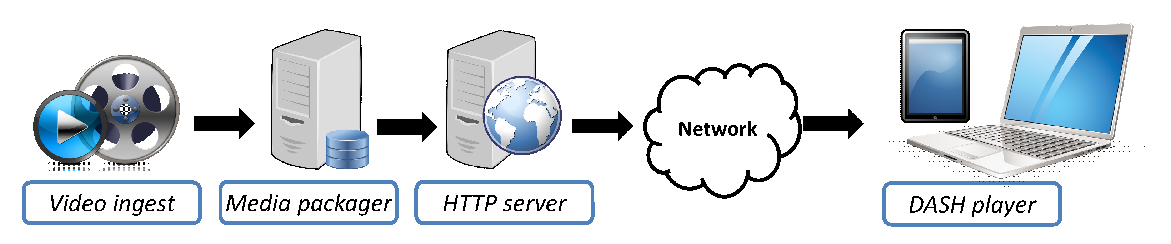
\includegraphics[width=1\textwidth,keepaspectratio]{system.eps}
	\caption{End-to-End DASH streaming system.}
	\label{fig:BMSB2019system}
\end{figure}

Video ingest is the system which injects the content into the processing and delivery chain. Many and different entities can act as a live source for media production, e.g. a live camera or any video software editor.

Media Packager is based on GStreamer \cite{gstreamer}. It is in charge of processing the content ingested and generating a standard compliant Chunked CMAF MPEG DASH stream. It encodes the content, packetizes it into MP4 fragments and segments and creates a live DASH Media Presentation Description (MPD) to expose the stream to the clients. The recent stable GStreamer release (v1.14) does not provides capabilities for generating a Chunked CMAF steam. Then, to experiment with Chunked CMAF, we introduced additional features and properly tuned the following plugins based on GStreamer v1.5:

\begin{itemize}
	\item \textit{H264 encoder}: the performance and setup of the encoder is key to favour a low latency stream, enabling the player to request the last generated MP4 fragment and to start its playback. \textit{Keyframes} (I-frames) do not require any other frames to be decoded, so the player has to start decoding a stream from a \textit{keyframe}. Thus, \textit{keyframes} are essential for live streaming and each generated fragment should start with a \textit{keyframe} to boost the playback start. The Group of Pictures (GOP) is a collection of successive pictures within a coded video stream where the \textit{keyframe} always indicates the beginning of a GOP. In terms of header information, some fields are mandatory for playing the stream, e.g. Sequence Parameter Set (SPS) and Picture Parameter Set (PPS) provide basic parameters like the frame size. Consequently, we encode the content forcing the presence of a \textit{keyframe} and all the header information at the beginning of each MP4 fragment. Moreover, for the remaining frames we avoid to use bidirectional predicted frames (B-frames) since they add additional latency into the encoding process due to required frames reorder. The resulting stream contains only key and predicted frames (I-frames and P-frames).
	\item \textit{MP4 muxer}: it packetizes the encoded frames into MP4 fragments and segments. Since we established that each fragment contain only one GOP, with a \textit{keyframe} at the beginning, the muxer works by switching from a fragment to another each time it recognizes a \textit{keyframe} generated by the encoder. In case a minimum theoretical latency wants to be exercised, putting bandwidth efficiency aside for unlimited connectivity, the encoder could just use \textit{keyframes}, i.e. no predicted frames are used, meaning the MP4 fragment contains just one frame. According to the specifications, each fragment contains header information (moof) and a payload (mdat) with the encoded data.
	\item \textit{MPEG-DASH filesink}: it receives the MP4 fragments from the muxer and aggregates them in order to write the segments on the disk. Since the fragments can be decoded independently each other, the fragments are concatenated by appending the new fragment at the end of the previous one. Following this strategy, it is not necessary to receive all the fragments to start writing a segment, which is progressively written on the disk. The filesink also creates the MPD manifest which contains the URL where the player can download the last fragment or, in case of legacy live MPEG-DASH stream, the segment. The filesink also updates the \textit{availabilityStartTime} field of the MPD manifest to allow the player to calculate the last generated fragment (or segment) time with accuracy and to download it. The generated MPD and the segments are directly written by the filesink in the storage of the HTTP Server.
\end{itemize}


HTTP Server is based on Node.js \cite{nodejs}. It is in charge of serving the content generated by the Media Packager to the player. When the player connects to the HTTP Server, the server loads the content from its storage and serves each fragment promptly to the player. Its functions include:
\begin{enumerate}
	\item It loads partial segments which are still being generated by Media Packager.
	\item It analyzes a segment and recognizes the contained MP4 fragments.
	\item It serves the fragments to the client through HTTP 1.1 chunked transfer encoding. Each HTTP chunk contains one fragment.
	%\item In case the player requests are not perfectly synchronized and the required fragment is not available, it waits until the fragment is generated in order to serve it.
\end{enumerate}

DASH player is based on the last stable GStreamer release (v1.14) \cite{gstreamer}. This version already provides capabilities to parse the manifest and request the last generated segment, then decoding and displaying it. Thus, it is able to play legacy MPEG-DASH streams. Moreover, GStreamer HTTP source plugin is able to receive a HTTP 1.1 chunked response when using a fragmented segment, but it does not pass the downloaded fragments to the decoding pipeline until it receives the whole segment. Thus, this is not valid in case of low latency streaming and the implementation of a Chunked CMAF Media Packager and HTTP Server would not be applicable. On the contrary, the HTTP source can request a section of a file if the exact byte range of the fragment inside a segment is known. The player can request the fragments separately and forward it to the decoding pipeline. Consequently, we modify the capabilities of the Media Packager in order to add \textit{mediaRange} \cite{mediarange} attributes inside the manifest which explicitly provides the DASH Player the byte range of the fragment. The player parses this attribute and requests separately the fragments to the server by adding Range header \cite{range} into the HTTP 1.1 request. The HTTP Server receives the requests, analyzes the segment and send the fragment included in the chosen range. When the player receives the fragment, it forwards the fragment to the decoding pipeline. Furthermore, to reduce latency, it is also important to take into account the internal playout buffer at the player since it is a widely used mechanism for preventing image freezes. However, it adds delay when playing the content. To overcome this limitation, we tuned the buffer size to be equal to one fragment duration. Finally, to synchronize the player and calculate the last fragment time with accuracy, we employ the network time protocol (NTP) to keep the Media Packager at server side and player device at client side synchronized. To sum up, the player does the following tasks:
\begin{enumerate}
	\item It parses the MPD manifest in order to get the \textit{availabilityStartTime}
	\item It compares the \textit{availabiltyStartTime} with NTP clock time in order to know which is the last generated fragment or, in case of legacy MPEG-DASH stream, segment.
	\item It requests the last generated fragment (or segment) from the HTTP Server.
	\item It decodes and displays the received stream.
\end{enumerate}

The communication between the nodes of the system is shown in Figure \ref{fig:BMSB2019sequence}.

\begin{figure}[htp]
	\centering
	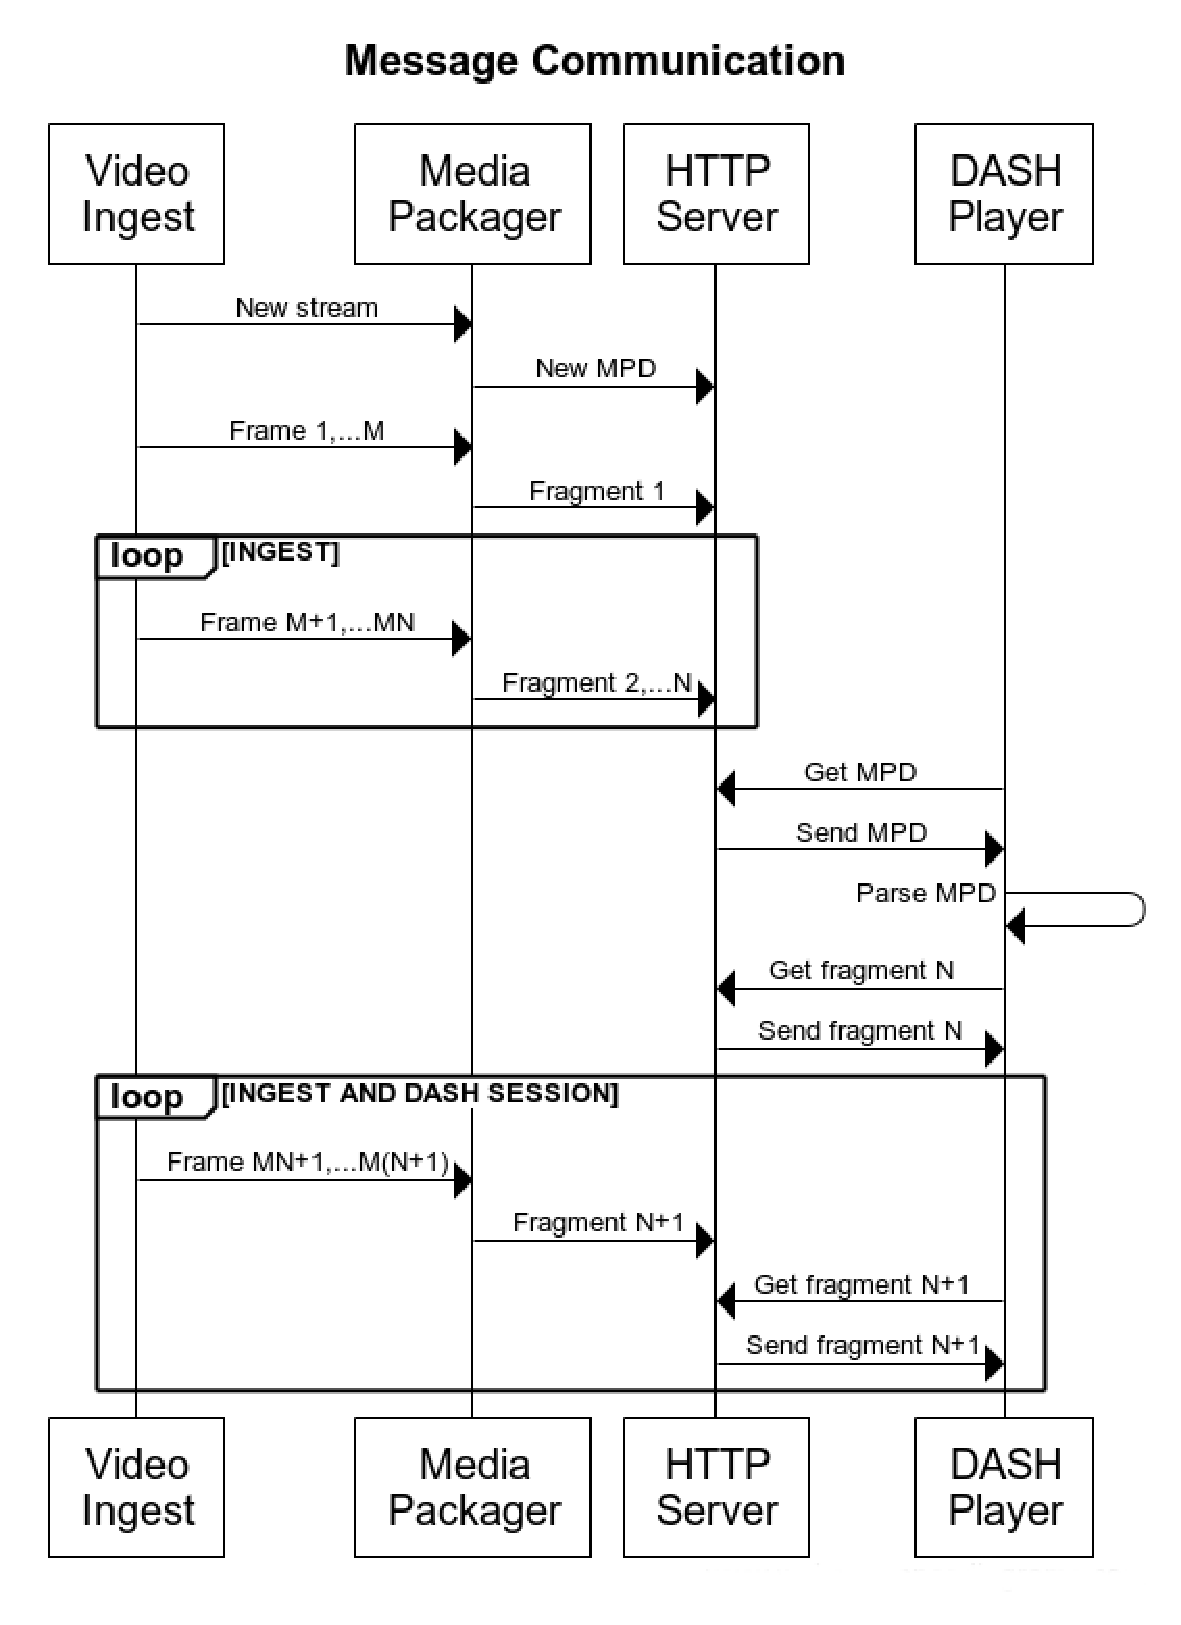
\includegraphics[width=0.7\textwidth,keepaspectratio]{webseq3.eps}
	\caption{Sequence diagram.}
	\label{fig:BMSB2019sequence}
\end{figure}

Media Packager begins to encode and packetize the content into MP4 fragments when the live source is connected.
The Chunked CMAF content is directly stored inside the storage located at the HTTP Server. Meanwhile the content is generated, the clients can connect to the HTTP Server which serves the segments.

\subsubsection{QoE Metrics}
\label{sec:BMSB2019measurement}

The measurements of the implemented solution aim to identify the effects on QoE. From the work of Claeys et al. \cite{claeys2014}, the QoE is related to objective metrics such as frequency and duration of freezes that we can measure directly introducing some probes into the player while playing the content. We consider that the playback freezes when the internal buffer of the player goes empty and defines the duration of the freeze the time between the buffer goes empty and it starts to refill.

Moreover, Hossfeld et al. \cite{hossfeld2012} investigates the effects of playout delay on the user and concludes that the user's satisfaction decreases while the playout delay increases. The playout is the elapsed time between the moment the user pushes the play button and the first frame is displayed on the screen. Anyway, in case of low latency, the playout depends also on content generation since the player needs to synchronize with sender. Consequently, in case of low latency steaming, it is more useful to measure the end-to-end latency of the system. From the work of Essaili et al. \cite{essaili2018}, the latency is the elapsed time between the frame ingest at the Media Packager (T$_{in}$) and the visualization time on the player screen (T$_{out}$), it can be express through the Expression \ref{eq:BMSB2019latency}.

\begin{equation}
\label{eq:BMSB2019latency}
Latency = T_{in} - T_{out} = T_{enc} + d_F + T_{fetch} + T_{dec}
\end{equation}

The latency depends on processing time at Media Packager (T$_{enc}$), the fragment duration (d$_F$), the time for fetching the fragment from HTTP Server (T$_{fetch}$) and the decoding time at the player (T$_{dec}$).

We evaluate the latency of the end-to-end system by summing up all the components which appear in the Equation (\ref{eq:BMSB2019latency}). Since in case of live streaming the Media Packager should work on real-time, T$_{enc}$ is inversely proportional to the input framerate. Accordingly, T$_{enc}$ is considered a fixed value. In the next section the remaining values of Equation (\ref{eq:BMSB2019latency}) are evaluated.

\subsection{Results}
\label{sec:BMSB2019results}

To test the implemented end-to-end Chunked CMAF solution, a live MPEG-DASH dataset using Big Buck Bunny test sequence was employed. Its raw version is provided by Xiph.Org Foundation \cite{xiph}. The raw video was encoded in H264/AVC format (ISO/IEC23008-2:2015). Then, it is multiplexed in ISO MPEG4 fragments (ISO / IEC 14496-12 - MPEG-4 Part 12) and split into segments. We experiment with the different representation levels shown in Table \ref{tab:BMSB2019reps}.

\begin{table}[htp]
	\caption{Set of MPEG-DASH representations employed in the experiments.}
	\centering
	\bgroup
	\def\arraystretch{1.2}%  1 is the default, change whatever you need
	\setlength\tabcolsep{2.5pt} % default value: 6pt
	\label{tab:BMSB2019reps}
	\def\arraystretch{1.2}%  1 is the default, change whatever you need
	\setlength\tabcolsep{2.0pt} % default value: 6pt
	{\scriptsize
		\begin{tabular}{>{\centering\arraybackslash}m{\dimexpr0.1\textwidth-2\tabcolsep-\arrayrulewidth\relax}
			>{\centering\arraybackslash}m{\dimexpr0.15\textwidth-2\tabcolsep-\arrayrulewidth\relax}
			>{\centering\arraybackslash}m{\dimexpr0.15\textwidth-2\tabcolsep-\arrayrulewidth\relax}
			>{\centering\arraybackslash}m{\dimexpr0.15\textwidth-2\tabcolsep-\arrayrulewidth\relax}
		}
		\toprule
		\textbf{Index} & \textbf{bitrate} & \textbf{resolution} & \textbf{framerate} \\
		\midrule
		\midrule
		1 & 1200kbps & 352x288 & 30fps  \\
		2 & 1600kbps & 640x360 & 30fps  \\
		3 & 2250kbps & 960x540 & 30fps \\
		4 & 2000kbps & 704x576 & 30fps \\
		5 & 4500kbps & 1280x720 & 30fps \\
		6 & 8000kbps & 1920x1080 & 30fps \\
		\bottomrule
		\bottomrule
	\end{tabular}
	\egroup
	}
\end{table}

Moreover, the tests were carried out using different fragment configurations settings while generating each representation level to compare a legacy MPEG-DASH live stream and a Chunked CMAF enabled one. In Table \ref{tab:BMSB2019tests} the employed fragment configurations are shown. The chosen duration for the segments along the tests is fixed to 2 seconds. This is a widely used value for legacy MPEG-DASH live streams, while the fragment duration employed is set to 33 ms, 100 ms or 167 ms for the Chunked CMAF live streams. These values correspond to fragments containing a GOP with 1, 3 or 5 frames, respectively.

\begin{table}[htp]
	\caption{Tested fragment configuration}
	\centering
	\bgroup
	\def\arraystretch{1.2}%  1 is the default, change whatever you need
	\setlength\tabcolsep{2.5pt} % default value: 6pt
	\label{tab:BMSB2019tests}
	\def\arraystretch{1.2}%  1 is the default, change whatever you need
	\setlength\tabcolsep{2.0pt} % default value: 6pt
	{\scriptsize
		\begin{tabular}{>{\centering\arraybackslash}m{\dimexpr0.1\textwidth-2\tabcolsep-\arrayrulewidth\relax}
			>{\centering\arraybackslash}m{\dimexpr0.15\textwidth-2\tabcolsep-\arrayrulewidth\relax}
			>{\centering\arraybackslash}m{\dimexpr0.15\textwidth-2\tabcolsep-\arrayrulewidth\relax}
		}
		\toprule
		\textbf{ID} & \textbf{Frames per fragment} & \textbf{Fragment duration (d$_F$) (ms)} \\
		\midrule
		\midrule
		F$_1$ & 1 & 33\\
		F$_3$ & 3 & 100\\
		F$_5$ & 5 & 167\\
		S (Legacy) & 60 & 2000\\
		\bottomrule
		\bottomrule
	\end{tabular}
	\egroup
	}
\end{table}

The experimental setup employed for the executed tests is presented in Figure \ref{fig:BMSB2019setup}. The overall setup comprises the following nodes:
\begin{itemize}
	\item Server: this node is in charge of creating and distributing the content, i.e. it runs both the Media Packager and the HTTP Server. It creates the live stream and serves it to the client when required by the client itself.
	\item Wireless access point: to provide wireless capabilities, an access point is used, which provides a wireless local area network (WLAN) using 2.4 GHz band. The only role of the access point consists in forwarding all the incoming traffic on both sides (server and player).
	\item Player: a wireless network node connected to the access point, which is running the DASH Players. It uses probes in order to collect network information and player internal status.
\end{itemize}

\begin{figure}[htp]
	\centering
	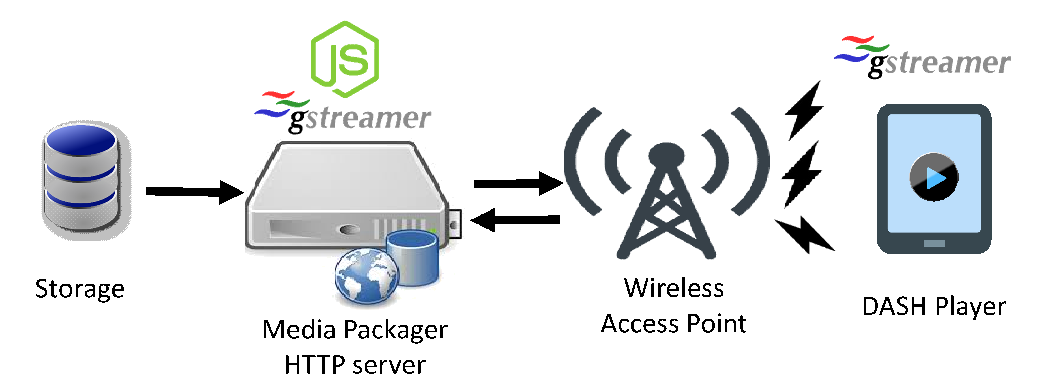
\includegraphics[width=1\textwidth,keepaspectratio]{setup.eps}
	\caption{Experimental setup.}
	\label{fig:BMSB2019setup}
\end{figure}

The Table \ref{tab:BMSB2019results} shows the results for the different fragment configurations and the employed representations in terms of the number of freezes and their average duration, and the overall latency according to the Equation (\ref{eq:BMSB2019latency}). These parameters are the common factors employed by \cite{claeys2014, hossfeld2012} for the assessment of MOS metrics.

\begin{table}[htp]
	\caption{Number of freezes (F$_{Nb}$), average freeze duration (F$_{avg}$) for each fragment configuration.}
	\centering
	\def\arraystretch{1.2}%  1 is the default, change whatever you need
	\setlength\tabcolsep{2.5pt} % default value: 6pt
	\label{tab:BMSB2019results}
	{\scriptsize
		\begin{tabular}{>{\centering\arraybackslash}m{\dimexpr0.1\textwidth-2\tabcolsep-\arrayrulewidth\relax}
				>{\centering\arraybackslash}m{\dimexpr0.1\textwidth-2\tabcolsep-\arrayrulewidth\relax}
				>{\centering\arraybackslash}m{\dimexpr0.1\textwidth-2\tabcolsep-\arrayrulewidth\relax}
				>{\centering\arraybackslash}m{\dimexpr0.1\textwidth-2\tabcolsep-\arrayrulewidth\relax}
				>{\centering\arraybackslash}m{\dimexpr0.1\textwidth-2\tabcolsep-\arrayrulewidth\relax}
			}
			\toprule
			\textbf{Conf.} & \textbf{Rep.} & \textbf{F$_{\textbf{Nb}}$} & \textbf{F$_{\textbf{avg}}$} & \textbf{Latency}\\
			\textbf{ID} & \textbf{index} & & \textbf{(ms)} & \textbf{(ms)} \\
			\midrule
			\midrule
			F$_1$ & 1 & 34 & 423 & 117\\
			F$_1$ & 2 & 35 & 410 & 124\\
			F$_1$ & 3 & 38 & 401 & 116\\
			F$_1$ & 4 & 30 & 466 & 117\\
			F$_1$ & 5 & 31 & 434 & 120\\
			F$_1$ & 6 & 13 & 445 & 126\\
			\bottomrule
			\bottomrule
		\end{tabular}
		\begin{tabular}{>{\centering\arraybackslash}m{\dimexpr0.1\textwidth-2\tabcolsep-\arrayrulewidth\relax}
			>{\centering\arraybackslash}m{\dimexpr0.1\textwidth-2\tabcolsep-\arrayrulewidth\relax}
			>{\centering\arraybackslash}m{\dimexpr0.1\textwidth-2\tabcolsep-\arrayrulewidth\relax}
			>{\centering\arraybackslash}m{\dimexpr0.1\textwidth-2\tabcolsep-\arrayrulewidth\relax}
			>{\centering\arraybackslash}m{\dimexpr0.1\textwidth-2\tabcolsep-\arrayrulewidth\relax}
		}
		\toprule
		\textbf{Conf.} & \textbf{Rep.} & \textbf{F$_{\textbf{Nb}}$} & \textbf{F$_{\textbf{avg}}$} & \textbf{Latency}\\
		\textbf{ID} & \textbf{index} & & \textbf{(ms)} & \textbf{(ms)} \\
		\midrule
		\midrule
		F$_3$ & 1 & 9 & 300 & 184\\
		F$_3$ & 2 & 3 & 492 & 187\\
		F$_3$ & 3 & 4 & 332 & 186\\
		F$_3$ & 4 & 9 & 294 & 186\\
		F$_3$ & 5 & 6 & 346 & 198\\
		F$_3$ & 6 & 11 & 401 & 222\\
		\bottomrule
		\bottomrule
		\end{tabular}
		\begin{tabular}{>{\centering\arraybackslash}m{\dimexpr0.1\textwidth-2\tabcolsep-\arrayrulewidth\relax}
			>{\centering\arraybackslash}m{\dimexpr0.1\textwidth-2\tabcolsep-\arrayrulewidth\relax}
			>{\centering\arraybackslash}m{\dimexpr0.1\textwidth-2\tabcolsep-\arrayrulewidth\relax}
			>{\centering\arraybackslash}m{\dimexpr0.1\textwidth-2\tabcolsep-\arrayrulewidth\relax}
			>{\centering\arraybackslash}m{\dimexpr0.1\textwidth-2\tabcolsep-\arrayrulewidth\relax}
		}
		\toprule
		\textbf{Conf.} & \textbf{Rep.} & \textbf{F$_{\textbf{Nb}}$} & \textbf{F$_{\textbf{avg}}$} & \textbf{Latency}\\
		\textbf{ID} & \textbf{index} & & \textbf{(ms)} & \textbf{(ms)} \\
		\midrule
		\midrule
		F$_5$ & 1 & 4 & 452 & 249\\
		F$_5$ & 2 & 14 & 312 & 256\\
		F$_5$ & 3 & 5 & 380 & 262\\
		F$_5$ & 4 & 5 & 493 & 259\\
		F$_5$ & 5 & 12 & 432 & 285\\
		F$_5$ & 6 & 13 & 430 & 317\\
		\bottomrule
		\bottomrule
		\end{tabular}
		\begin{tabular}{>{\centering\arraybackslash}m{\dimexpr0.1\textwidth-2\tabcolsep-\arrayrulewidth\relax}
			>{\centering\arraybackslash}m{\dimexpr0.1\textwidth-2\tabcolsep-\arrayrulewidth\relax}
			>{\centering\arraybackslash}m{\dimexpr0.1\textwidth-2\tabcolsep-\arrayrulewidth\relax}
			>{\centering\arraybackslash}m{\dimexpr0.1\textwidth-2\tabcolsep-\arrayrulewidth\relax}
			>{\centering\arraybackslash}m{\dimexpr0.1\textwidth-2\tabcolsep-\arrayrulewidth\relax}
		}
		\toprule
		\textbf{Conf.} & \textbf{Rep.} & \textbf{F$_{\textbf{Nb}}$} & \textbf{F$_{\textbf{avg}}$} & \textbf{Latency}\\
		\textbf{ID} & \textbf{index} & & \textbf{(ms)} & \textbf{(ms)} \\
		\midrule
		\midrule
		S & 1 & 0 & - & 2196\\
		S & 2 & 0 & - & 2231\\
		S & 3 & 0 & - & 2288\\
		S & 4 & 0 & - & 2261\\
		S & 5 & 0 & - & 2482\\
		S & 6 & 2 & 463 & 2196\\
		\bottomrule
		\bottomrule
		\end{tabular}
	}
\end{table}

It becomes clear that the reduction of the fragment duration means a reduction in latency, but it also increases the number of freezes as the network performance is not enough to deliver the fragments in time. The duration of each freeze is not related to the fragment duration as the freezes spans a duration between 300 and 400 milliseconds independently of the fragment duration. Thus, it looks like an intrinsic limit of the wireless setup. The configuration S (legacy) is the only one which is not affected by the freezes, except for the highest representation level. In any case, even when higher network resources are needed, the playout buffer is big enough to shield against any network fluctuation. As expected, the configuration F1 (1 frame per fragment) provides the lowest latency. However, the latency score is not exactly proportional to the GOP size since the latency reduction means -38\% compared to F3 (3 frames per segment) while theoretically latency should decrease 3 times. This effect is mainly produced by two factors. First, the increasing HTTP overheads when the request/response speed and volume is very high. Second, the higher data rates to be transferred due to the utilization of more keyframes meaning high bitrates and lower compression efficiency as a GOP needs to start with a keyframe to allow instant consumption of a live stream. Moreover, the number of freezes for configuration F1 is three times compared to F3 and F5 (5 frames per fragment), which means that, the maximum technical reduction of latency may significantly damage the user's QoE with higher freezes along streaming sessions.

\begin{figure}[htp]
	\centering
	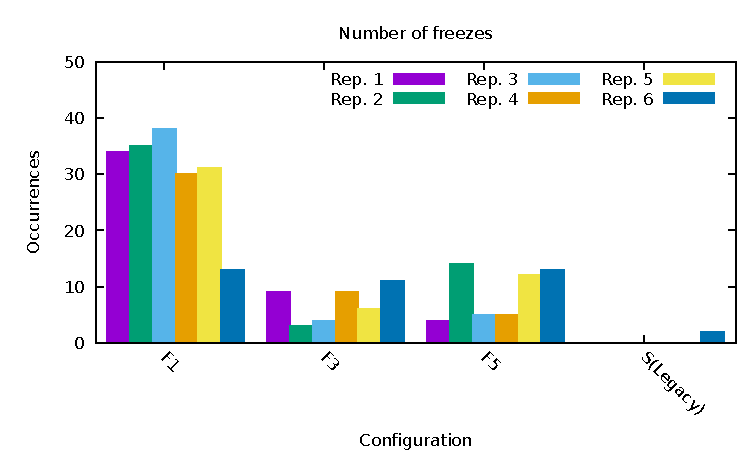
\includegraphics[width=1\textwidth,keepaspectratio]{freezes.eps}
	\caption{Number of freezes.}
	\label{fig:BMSB2019freezes}
\end{figure}

The results in terms of number of freezes along the video playback are presented in Figure \ref{fig:BMSB2019freezes}, comparing the occurrence for the different representations and fragment configurations. It is visually evident that the number of freezes is lower as the fragment duration is higher. Finally, the configuration F3 and F5 present almost the same number of freezes and duration and then F3 is preferable in order to reduce latency.

\subsection{Conclusions and Future Work}
\label{sec:BMSB2019conlusion}
This paper proposes an end-to-end system for delivery contents though a Chunked CMAF enabled MPEG-DASH live stream which aims to reduce latency, while trying to preserve major parameters of user's QoE.

The proposed solution has been integrated with Open Source MPEG-DASH framework and tested by performing experiments though a real testbed. The target of the experiments is the evaluation of the effects on user's QoE while tuning GOP and fragment duration during the Chunked CMAF packetizing in order to vary the latency of the system.

The results show that DASH players gain lower latency in any of the Chunked CMAF configuration with respects to a legacy solution but when using an aggressive configuration with a small GOP size and fragment duration the playback is frequently affected by freezes which reduce the QoE. So, to balance the latency and QoE trade-off a more conservative configuration of Chunked CMAF is suggested.


% use section* for acknowledgement
%\subsection*{Acknowledgment}





